\documentclass[1p]{elsarticle_modified}
%\bibliographystyle{elsarticle-num}

%\usepackage[colorlinks]{hyperref}
%\usepackage{abbrmath_seonhwa} %\Abb, \Ascr, \Acal ,\Abf, \Afrak
\usepackage{amsfonts}
\usepackage{amssymb}
\usepackage{amsmath}
\usepackage{amsthm}
\usepackage{scalefnt}
\usepackage{amsbsy}
\usepackage{kotex}
\usepackage{caption}
\usepackage{subfig}
\usepackage{color}
\usepackage{graphicx}
\usepackage{xcolor} %% white, black, red, green, blue, cyan, magenta, yellow
\usepackage{float}
\usepackage{setspace}
\usepackage{hyperref}

\usepackage{tikz}
\usetikzlibrary{arrows}

\usepackage{multirow}
\usepackage{array} % fixed length table
\usepackage{hhline}

%%%%%%%%%%%%%%%%%%%%%
\makeatletter
\renewcommand*\env@matrix[1][\arraystretch]{%
	\edef\arraystretch{#1}%
	\hskip -\arraycolsep
	\let\@ifnextchar\new@ifnextchar
	\array{*\c@MaxMatrixCols c}}
\makeatother %https://tex.stackexchange.com/questions/14071/how-can-i-increase-the-line-spacing-in-a-matrix
%%%%%%%%%%%%%%%

\usepackage[normalem]{ulem}

\newcommand{\msout}[1]{\ifmmode\text{\sout{\ensuremath{#1}}}\else\sout{#1}\fi}
%SOURCE: \msout is \stkout macro in https://tex.stackexchange.com/questions/20609/strikeout-in-math-mode

\newcommand{\cancel}[1]{
	\ifmmode
	{\color{red}\msout{#1}}
	\else
	{\color{red}\sout{#1}}
	\fi
}

\newcommand{\add}[1]{
	{\color{blue}\uwave{#1}}
}

\newcommand{\replace}[2]{
	\ifmmode
	{\color{red}\msout{#1}}{\color{blue}\uwave{#2}}
	\else
	{\color{red}\sout{#1}}{\color{blue}\uwave{#2}}
	\fi
}

\newcommand{\Sol}{\mathcal{S}} %segment
\newcommand{\D}{D} %diagram
\newcommand{\A}{\mathcal{A}} %arc


%%%%%%%%%%%%%%%%%%%%%%%%%%%%%5 test

\def\sl{\operatorname{\textup{SL}}(2,\Cbb)}
\def\psl{\operatorname{\textup{PSL}}(2,\Cbb)}
\def\quan{\mkern 1mu \triangleright \mkern 1mu}

\theoremstyle{definition}
\newtheorem{thm}{Theorem}[section]
\newtheorem{prop}[thm]{Proposition}
\newtheorem{lem}[thm]{Lemma}
\newtheorem{ques}[thm]{Question}
\newtheorem{cor}[thm]{Corollary}
\newtheorem{defn}[thm]{Definition}
\newtheorem{exam}[thm]{Example}
\newtheorem{rmk}[thm]{Remark}
\newtheorem{alg}[thm]{Algorithm}

\newcommand{\I}{\sqrt{-1}}
\begin{document}

%\begin{frontmatter}
%
%\title{Boundary parabolic representations of knots up to 8 crossings}
%
%%% Group authors per affiliation:
%\author{Yunhi Cho} 
%\address{Department of Mathematics, University of Seoul, Seoul, Korea}
%\ead{yhcho@uos.ac.kr}
%
%
%\author{Seonhwa Kim} %\fnref{s_kim}}
%\address{Center for Geometry and Physics, Institute for Basic Science, Pohang, 37673, Korea}
%\ead{ryeona17@ibs.re.kr}
%
%\author{Hyuk Kim}
%\address{Department of Mathematical Sciences, Seoul National University, Seoul 08826, Korea}
%\ead{hyukkim@snu.ac.kr}
%
%\author{Seokbeom Yoon}
%\address{Department of Mathematical Sciences, Seoul National University, Seoul, 08826,  Korea}
%\ead{sbyoon15@snu.ac.kr}
%
%\begin{abstract}
%We find all boundary parabolic representation of knots up to 8 crossings.
%
%\end{abstract}
%\begin{keyword}
%    \MSC[2010] 57M25 
%\end{keyword}
%
%\end{frontmatter}

%\linenumbers
%\tableofcontents
%
\newcommand\colored[1]{\textcolor{white}{\rule[-0.35ex]{0.8em}{1.4ex}}\kern-0.8em\color{red} #1}%
%\newcommand\colored[1]{\textcolor{white}{ #1}\kern-2.17ex	\textcolor{white}{ #1}\kern-1.81ex	\textcolor{white}{ #1}\kern-2.15ex\color{red}#1	}

{\Large $\underline{12a_{0680}~(K12a_{0680})}$}

\setlength{\tabcolsep}{10pt}
\renewcommand{\arraystretch}{1.6}
\vspace{1cm}\begin{tabular}{m{100pt}>{\centering\arraybackslash}m{274pt}}
\multirow{5}{120pt}{
	\centering
	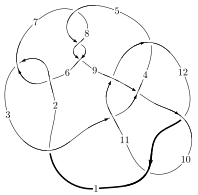
\includegraphics[width=112pt]{../../../GIT/diagram.site/Diagrams/png/1481_12a_0680.png}\\
\ \ \ A knot diagram\footnotemark}&
\allowdisplaybreaks
\textbf{Linearized knot diagam} \\
\cline{2-2}
 &
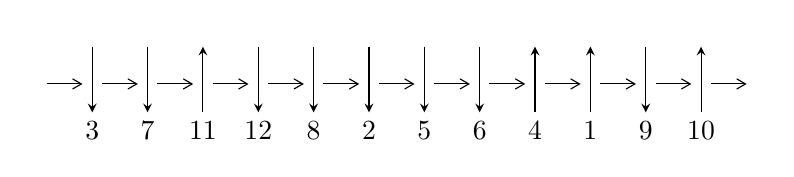
\begin{tikzpicture}[x=20pt, y=17pt]
	% nodes
	\node (C0) at (0, 0) {};
	\node (C1) at (1, 0) {};
	\node (C1U) at (1, +1) {};
	\node (C1D) at (1, -1) {3};

	\node (C2) at (2, 0) {};
	\node (C2U) at (2, +1) {};
	\node (C2D) at (2, -1) {7};

	\node (C3) at (3, 0) {};
	\node (C3U) at (3, +1) {};
	\node (C3D) at (3, -1) {11};

	\node (C4) at (4, 0) {};
	\node (C4U) at (4, +1) {};
	\node (C4D) at (4, -1) {12};

	\node (C5) at (5, 0) {};
	\node (C5U) at (5, +1) {};
	\node (C5D) at (5, -1) {8};

	\node (C6) at (6, 0) {};
	\node (C6U) at (6, +1) {};
	\node (C6D) at (6, -1) {2};

	\node (C7) at (7, 0) {};
	\node (C7U) at (7, +1) {};
	\node (C7D) at (7, -1) {5};

	\node (C8) at (8, 0) {};
	\node (C8U) at (8, +1) {};
	\node (C8D) at (8, -1) {6};

	\node (C9) at (9, 0) {};
	\node (C9U) at (9, +1) {};
	\node (C9D) at (9, -1) {4};

	\node (C10) at (10, 0) {};
	\node (C10U) at (10, +1) {};
	\node (C10D) at (10, -1) {1};

	\node (C11) at (11, 0) {};
	\node (C11U) at (11, +1) {};
	\node (C11D) at (11, -1) {9};

	\node (C12) at (12, 0) {};
	\node (C12U) at (12, +1) {};
	\node (C12D) at (12, -1) {10};
	\node (C13) at (13, 0) {};

	% arrows
	\draw[->,>={angle 60}]
	(C0) edge (C1) (C1) edge (C2) (C2) edge (C3) (C3) edge (C4) (C4) edge (C5) (C5) edge (C6) (C6) edge (C7) (C7) edge (C8) (C8) edge (C9) (C9) edge (C10) (C10) edge (C11) (C11) edge (C12) (C12) edge (C13) ;	\draw[->,>=stealth]
	(C1U) edge (C1D) (C2U) edge (C2D) (C3D) edge (C3U) (C4U) edge (C4D) (C5U) edge (C5D) (C6U) edge (C6D) (C7U) edge (C7D) (C8U) edge (C8D) (C9D) edge (C9U) (C10D) edge (C10U) (C11U) edge (C11D) (C12D) edge (C12U) ;
	\end{tikzpicture} \\
\hhline{~~} \\& 
\textbf{Solving Sequence} \\ \cline{2-2} 
 &
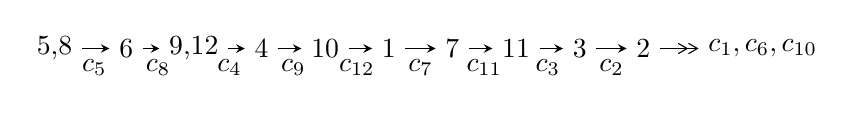
\begin{tikzpicture}[x=23pt, y=7pt]
	% node
	\node (A0) at (-1/8, 0) {5,8};
	\node (A1) at (1, 0) {6};
	\node (A2) at (33/16, 0) {9,12};
	\node (A3) at (25/8, 0) {4};
	\node (A4) at (33/8, 0) {10};
	\node (A5) at (41/8, 0) {1};
	\node (A6) at (49/8, 0) {7};
	\node (A7) at (57/8, 0) {11};
	\node (A8) at (65/8, 0) {3};
	\node (A9) at (73/8, 0) {2};
	\node (C1) at (1/2, -1) {$c_{5}$};
	\node (C2) at (3/2, -1) {$c_{8}$};
	\node (C3) at (21/8, -1) {$c_{4}$};
	\node (C4) at (29/8, -1) {$c_{9}$};
	\node (C5) at (37/8, -1) {$c_{12}$};
	\node (C6) at (45/8, -1) {$c_{7}$};
	\node (C7) at (53/8, -1) {$c_{11}$};
	\node (C8) at (61/8, -1) {$c_{3}$};
	\node (C9) at (69/8, -1) {$c_{2}$};
	\node (A10) at (11, 0) {$c_{1},c_{6},c_{10}$};

	% edge
	\draw[->,>=stealth]	
	(A0) edge (A1) (A1) edge (A2) (A2) edge (A3) (A3) edge (A4) (A4) edge (A5) (A5) edge (A6) (A6) edge (A7) (A7) edge (A8) (A8) edge (A9) ;
	\draw[->>,>={angle 60}]	
	(A9) edge (A10);
\end{tikzpicture} \\ 

\end{tabular} \\

\footnotetext{
The image of knot diagram is generated by the software ``\textbf{Draw programme}" developed by Andrew Bartholomew(\url{http://www.layer8.co.uk/maths/draw/index.htm\#Running-draw}), where we modified some parts for our purpose(\url{https://github.com/CATsTAILs/LinksPainter}).
}\phantom \\ \newline 
\centering \textbf{Ideals for irreducible components\footnotemark of $X_{\text{par}}$} 
 
\begin{align*}
I^u_{1}&=\langle 
2.30506\times10^{89} u^{105}+1.23026\times10^{90} u^{104}+\cdots+1.08124\times10^{88} b+1.22301\times10^{89},\\
\phantom{I^u_{1}}&\phantom{= \langle  }-6.32954\times10^{88} u^{105}-3.69628\times10^{89} u^{104}+\cdots+2.70309\times10^{87} a-6.48561\times10^{88},\;u^{106}+7 u^{105}+\cdots- u^2+1\rangle \\
I^u_{2}&=\langle 
-2 a^4-9 a^3-10 a^2+5 b-11 a-4,\;a^5+5 a^4+6 a^3+3 a^2+a+1,\;u-1\rangle \\
I^u_{3}&=\langle 
b+u+2,\;a-2 u-3,\;u^2+u-1\rangle \\
\\
\end{align*}
\raggedright * 3 irreducible components of $\dim_{\mathbb{C}}=0$, with total 113 representations.\\
\footnotetext{All coefficients of polynomials are rational numbers. But the coefficients are sometimes approximated in decimal forms when there is not enough margin.}
\newpage
\renewcommand{\arraystretch}{1}
\centering \section*{I. $I^u_{1}= \langle 2.31\times10^{89} u^{105}+1.23\times10^{90} u^{104}+\cdots+1.08\times10^{88} b+1.22\times10^{89},\;-6.33\times10^{88} u^{105}-3.70\times10^{89} u^{104}+\cdots+2.70\times10^{87} a-6.49\times10^{88},\;u^{106}+7 u^{105}+\cdots- u^2+1 \rangle$}
\flushleft \textbf{(i) Arc colorings}\\
\begin{tabular}{m{7pt} m{180pt} m{7pt} m{180pt} }
\flushright $a_{5}=$&$\begin{pmatrix}1\\0\end{pmatrix}$ \\
\flushright $a_{8}=$&$\begin{pmatrix}0\\u\end{pmatrix}$ \\
\flushright $a_{6}=$&$\begin{pmatrix}1\\u^2\end{pmatrix}$ \\
\flushright $a_{9}=$&$\begin{pmatrix}- u\\- u^3+u\end{pmatrix}$ \\
\flushright $a_{12}=$&$\begin{pmatrix}23.4159 u^{105}+136.742 u^{104}+\cdots-46.1677 u+23.9933\\-21.3187 u^{105}-113.783 u^{104}+\cdots+3.78375 u-11.3113\end{pmatrix}$ \\
\flushright $a_{4}=$&$\begin{pmatrix}-251.012 u^{105}-1411.63 u^{104}+\cdots+127.509 u-179.204\\-241.071 u^{105}-1355.21 u^{104}+\cdots+127.389 u-176.226\end{pmatrix}$ \\
\flushright $a_{10}=$&$\begin{pmatrix}65.9369 u^{105}+378.466 u^{104}+\cdots-60.0074 u+53.8430\\23.5122 u^{105}+140.434 u^{104}+\cdots-18.7637 u+22.2506\end{pmatrix}$ \\
\flushright $a_{1}=$&$\begin{pmatrix}-91.6179 u^{105}-515.563 u^{104}+\cdots+31.6304 u-63.6344\\-95.0632 u^{105}-536.170 u^{104}+\cdots+47.1533 u-69.1269\end{pmatrix}$ \\
\flushright $a_{7}=$&$\begin{pmatrix}u\\u\end{pmatrix}$ \\
\flushright $a_{11}=$&$\begin{pmatrix}-37.2311 u^{105}-201.840 u^{104}+\cdots-16.8240 u-18.5106\\-81.3556 u^{105}-452.020 u^{104}+\cdots+35.0871 u-54.7541\end{pmatrix}$ \\
\flushright $a_{3}=$&$\begin{pmatrix}72.6372 u^{105}+410.221 u^{104}+\cdots-24.5715 u+50.5987\\127.336 u^{105}+721.871 u^{104}+\cdots-67.1446 u+94.7937\end{pmatrix}$ \\
\flushright $a_{2}=$&$\begin{pmatrix}166.039 u^{105}+941.534 u^{104}+\cdots-79.2707 u+121.844\\220.738 u^{105}+1253.18 u^{104}+\cdots-121.844 u+166.039\end{pmatrix}$\\&\end{tabular}
\flushleft \textbf{(ii) Obstruction class $= -1$}\\~\\
\flushleft \textbf{(iii) Cusp Shapes $= 117.650 u^{105}+684.548 u^{104}+\cdots-74.1017 u+98.6648$}\\~\\
\newpage\renewcommand{\arraystretch}{1}
\flushleft \textbf{(iv) u-Polynomials at the component}\newline \\
\begin{tabular}{m{50pt}|m{274pt}}
Crossings & \hspace{64pt}u-Polynomials at each crossing \\
\hline $$\begin{aligned}c_{1}\end{aligned}$$&$\begin{aligned}
&u^{106}+36 u^{105}+\cdots+15872 u+1024
\end{aligned}$\\
\hline $$\begin{aligned}c_{2},c_{6}\end{aligned}$$&$\begin{aligned}
&u^{106}-2 u^{105}+\cdots-32 u-32
\end{aligned}$\\
\hline $$\begin{aligned}c_{3}\end{aligned}$$&$\begin{aligned}
&u^{106}+u^{105}+\cdots+294900 u-153931
\end{aligned}$\\
\hline $$\begin{aligned}c_{4}\end{aligned}$$&$\begin{aligned}
&u^{106}+5 u^{105}+\cdots+117392 u+6541
\end{aligned}$\\
\hline $$\begin{aligned}c_{5},c_{7},c_{8}\end{aligned}$$&$\begin{aligned}
&u^{106}-7 u^{105}+\cdots- u^2+1
\end{aligned}$\\
\hline $$\begin{aligned}c_{9}\end{aligned}$$&$\begin{aligned}
&u^{106}+9 u^{105}+\cdots-2 u-1
\end{aligned}$\\
\hline $$\begin{aligned}c_{10},c_{12}\end{aligned}$$&$\begin{aligned}
&u^{106}+4 u^{105}+\cdots+63 u+1
\end{aligned}$\\
\hline $$\begin{aligned}c_{11}\end{aligned}$$&$\begin{aligned}
&u^{106}-18 u^{105}+\cdots-64 u+4
\end{aligned}$\\
\hline
\end{tabular}\\~\\
\newpage\renewcommand{\arraystretch}{1}
\flushleft \textbf{(v) Riley Polynomials at the component}\newline \\
\begin{tabular}{m{50pt}|m{274pt}}
Crossings & \hspace{64pt}Riley Polynomials at each crossing \\
\hline $$\begin{aligned}c_{1}\end{aligned}$$&$\begin{aligned}
&y^{106}+60 y^{105}+\cdots-50987008 y+1048576
\end{aligned}$\\
\hline $$\begin{aligned}c_{2},c_{6}\end{aligned}$$&$\begin{aligned}
&y^{106}-36 y^{105}+\cdots-15872 y+1024
\end{aligned}$\\
\hline $$\begin{aligned}c_{3}\end{aligned}$$&$\begin{aligned}
&y^{106}+47 y^{105}+\cdots-1112070735948 y+23694752761
\end{aligned}$\\
\hline $$\begin{aligned}c_{4}\end{aligned}$$&$\begin{aligned}
&y^{106}+119 y^{105}+\cdots-11945791032 y+42784681
\end{aligned}$\\
\hline $$\begin{aligned}c_{5},c_{7},c_{8}\end{aligned}$$&$\begin{aligned}
&y^{106}-89 y^{105}+\cdots-2 y+1
\end{aligned}$\\
\hline $$\begin{aligned}c_{9}\end{aligned}$$&$\begin{aligned}
&y^{106}-25 y^{105}+\cdots-20 y+1
\end{aligned}$\\
\hline $$\begin{aligned}c_{10},c_{12}\end{aligned}$$&$\begin{aligned}
&y^{106}-80 y^{105}+\cdots-5699 y+1
\end{aligned}$\\
\hline $$\begin{aligned}c_{11}\end{aligned}$$&$\begin{aligned}
&y^{106}+18 y^{105}+\cdots-888 y+16
\end{aligned}$\\
\hline
\end{tabular}\\~\\
\newpage\flushleft \textbf{(vi) Complex Volumes and Cusp Shapes}
$$\begin{array}{c|c|c}  
\text{Solutions to }I^u_{1}& \I (\text{vol} + \sqrt{-1}CS) & \text{Cusp shape}\\
 \hline 
\begin{aligned}
u &= \phantom{-}0.676515 + 0.691802 I \\
a &= -0.336335 - 0.448876 I \\
b &= \phantom{-}0.707004 - 0.745975 I\end{aligned}
 & \phantom{-}0.39517 + 2.43050 I & \phantom{-0.000000 } 0 \\ \hline\begin{aligned}
u &= \phantom{-}0.676515 - 0.691802 I \\
a &= -0.336335 + 0.448876 I \\
b &= \phantom{-}0.707004 + 0.745975 I\end{aligned}
 & \phantom{-}0.39517 - 2.43050 I & \phantom{-0.000000 } 0 \\ \hline\begin{aligned}
u &= \phantom{-}0.155047 + 0.936670 I \\
a &= -0.503729 + 0.426978 I \\
b &= -0.094660 - 0.739124 I\end{aligned}
 & \phantom{-}6.24033 - 5.37724 I & \phantom{-0.000000 } 0 \\ \hline\begin{aligned}
u &= \phantom{-}0.155047 - 0.936670 I \\
a &= -0.503729 - 0.426978 I \\
b &= -0.094660 + 0.739124 I\end{aligned}
 & \phantom{-}6.24033 + 5.37724 I & \phantom{-0.000000 } 0 \\ \hline\begin{aligned}
u &= \phantom{-}0.154727 + 0.905545 I \\
a &= \phantom{-}0.479403 - 1.199780 I \\
b &= \phantom{-}0.94668 + 1.37587 I\end{aligned}
 & \phantom{-}7.1033 - 13.7991 I & \phantom{-0.000000 } 0 \\ \hline\begin{aligned}
u &= \phantom{-}0.154727 - 0.905545 I \\
a &= \phantom{-}0.479403 + 1.199780 I \\
b &= \phantom{-}0.94668 - 1.37587 I\end{aligned}
 & \phantom{-}7.1033 + 13.7991 I & \phantom{-0.000000 } 0 \\ \hline\begin{aligned}
u &= \phantom{-}0.545270 + 0.721728 I \\
a &= \phantom{-}0.614138 - 0.509648 I \\
b &= \phantom{-}0.857426 + 0.932428 I\end{aligned}
 & \phantom{-}0.75431 - 7.41963 I & \phantom{-0.000000 } 0 \\ \hline\begin{aligned}
u &= \phantom{-}0.545270 - 0.721728 I \\
a &= \phantom{-}0.614138 + 0.509648 I \\
b &= \phantom{-}0.857426 - 0.932428 I\end{aligned}
 & \phantom{-}0.75431 + 7.41963 I & \phantom{-0.000000 } 0 \\ \hline\begin{aligned}
u &= \phantom{-}0.900430\phantom{ +0.000000I} \\
a &= -5.58526\phantom{ +0.000000I} \\
b &= \phantom{-}1.50828\phantom{ +0.000000I}\end{aligned}
 & \phantom{-}0.491361\phantom{ +0.000000I} & \phantom{-0.000000 } 0 \\ \hline\begin{aligned}
u &= \phantom{-}1.086680 + 0.311551 I \\
a &= -0.488568 - 0.839468 I \\
b &= \phantom{-}0.502420 - 0.844012 I\end{aligned}
 & -0.608988 - 0.539453 I & \phantom{-0.000000 } 0\\
 \hline 
 \end{array}$$\newpage$$\begin{array}{c|c|c}  
\text{Solutions to }I^u_{1}& \I (\text{vol} + \sqrt{-1}CS) & \text{Cusp shape}\\
 \hline 
\begin{aligned}
u &= \phantom{-}1.086680 - 0.311551 I \\
a &= -0.488568 + 0.839468 I \\
b &= \phantom{-}0.502420 + 0.844012 I\end{aligned}
 & -0.608988 + 0.539453 I & \phantom{-0.000000 } 0 \\ \hline\begin{aligned}
u &= -1.107130 + 0.281035 I \\
a &= -0.169385 + 0.289596 I \\
b &= -0.228945 + 1.090470 I\end{aligned}
 & \phantom{-}4.76987 + 4.98668 I & \phantom{-0.000000 } 0 \\ \hline\begin{aligned}
u &= -1.107130 - 0.281035 I \\
a &= -0.169385 - 0.289596 I \\
b &= -0.228945 - 1.090470 I\end{aligned}
 & \phantom{-}4.76987 - 4.98668 I & \phantom{-0.000000 } 0 \\ \hline\begin{aligned}
u &= \phantom{-}1.147060 + 0.071642 I \\
a &= -2.55732 - 0.51006 I \\
b &= -0.556726 - 1.145320 I\end{aligned}
 & -0.503326 - 1.106790 I & \phantom{-0.000000 } 0 \\ \hline\begin{aligned}
u &= \phantom{-}1.147060 - 0.071642 I \\
a &= -2.55732 + 0.51006 I \\
b &= -0.556726 + 1.145320 I\end{aligned}
 & -0.503326 + 1.106790 I & \phantom{-0.000000 } 0 \\ \hline\begin{aligned}
u &= \phantom{-}0.143266 + 0.836626 I \\
a &= -0.737577 + 1.002230 I \\
b &= -0.799361 - 0.878727 I\end{aligned}
 & \phantom{-}2.20961 - 7.79473 I & \phantom{-0.000000 } 0 \\ \hline\begin{aligned}
u &= \phantom{-}0.143266 - 0.836626 I \\
a &= -0.737577 - 1.002230 I \\
b &= -0.799361 + 0.878727 I\end{aligned}
 & \phantom{-}2.20961 + 7.79473 I & \phantom{-0.000000 } 0 \\ \hline\begin{aligned}
u &= \phantom{-}1.095120 + 0.407068 I \\
a &= -0.491541 + 0.367384 I \\
b &= -0.703204 + 0.844493 I\end{aligned}
 & -0.70354 + 3.31461 I & \phantom{-0.000000 } 0 \\ \hline\begin{aligned}
u &= \phantom{-}1.095120 - 0.407068 I \\
a &= -0.491541 - 0.367384 I \\
b &= -0.703204 - 0.844493 I\end{aligned}
 & -0.70354 - 3.31461 I & \phantom{-0.000000 } 0 \\ \hline\begin{aligned}
u &= \phantom{-}0.088609 + 0.814986 I \\
a &= -0.72225 - 1.64625 I \\
b &= -0.008950 + 0.823472 I\end{aligned}
 & \phantom{-}6.58986 - 4.90925 I & \phantom{-0.000000 } 0\\
 \hline 
 \end{array}$$\newpage$$\begin{array}{c|c|c}  
\text{Solutions to }I^u_{1}& \I (\text{vol} + \sqrt{-1}CS) & \text{Cusp shape}\\
 \hline 
\begin{aligned}
u &= \phantom{-}0.088609 - 0.814986 I \\
a &= -0.72225 + 1.64625 I \\
b &= -0.008950 - 0.823472 I\end{aligned}
 & \phantom{-}6.58986 + 4.90925 I & \phantom{-0.000000 } 0 \\ \hline\begin{aligned}
u &= -0.162273 + 0.798920 I \\
a &= \phantom{-}0.797320 + 0.306408 I \\
b &= -0.100735 - 0.852468 I\end{aligned}
 & \phantom{-}7.55362 - 0.96837 I & \phantom{-0.000000 } 0 \\ \hline\begin{aligned}
u &= -0.162273 - 0.798920 I \\
a &= \phantom{-}0.797320 - 0.306408 I \\
b &= -0.100735 + 0.852468 I\end{aligned}
 & \phantom{-}7.55362 + 0.96837 I & \phantom{-0.000000 } 0 \\ \hline\begin{aligned}
u &= -1.149890 + 0.305354 I \\
a &= \phantom{-}0.048581 - 0.495678 I \\
b &= -0.67876 - 1.36317 I\end{aligned}
 & \phantom{-}5.12337 - 3.69187 I & \phantom{-0.000000 } 0 \\ \hline\begin{aligned}
u &= -1.149890 - 0.305354 I \\
a &= \phantom{-}0.048581 + 0.495678 I \\
b &= -0.67876 + 1.36317 I\end{aligned}
 & \phantom{-}5.12337 + 3.69187 I & \phantom{-0.000000 } 0 \\ \hline\begin{aligned}
u &= \phantom{-}0.149263 + 0.789775 I \\
a &= -0.017817 - 0.679262 I \\
b &= \phantom{-}0.937147 + 0.817368 I\end{aligned}
 & \phantom{-}2.21730 - 3.52862 I & \phantom{-0.000000 } 0 \\ \hline\begin{aligned}
u &= \phantom{-}0.149263 - 0.789775 I \\
a &= -0.017817 + 0.679262 I \\
b &= \phantom{-}0.937147 - 0.817368 I\end{aligned}
 & \phantom{-}2.21730 + 3.52862 I & \phantom{-0.000000 } 0 \\ \hline\begin{aligned}
u &= -0.116906 + 0.784426 I \\
a &= -0.68138 - 1.33921 I \\
b &= -0.83302 + 1.34491 I\end{aligned}
 & \phantom{-}8.23030 + 7.68453 I & \phantom{-0.000000 } 0 \\ \hline\begin{aligned}
u &= -0.116906 - 0.784426 I \\
a &= -0.68138 + 1.33921 I \\
b &= -0.83302 - 1.34491 I\end{aligned}
 & \phantom{-}8.23030 - 7.68453 I & \phantom{-0.000000 } 0 \\ \hline\begin{aligned}
u &= \phantom{-}0.043513 + 0.784836 I \\
a &= \phantom{-}0.97448 - 1.51173 I \\
b &= \phantom{-}0.047337 + 0.690405 I\end{aligned}
 & \phantom{-}6.79678 - 0.76185 I & \phantom{-0.000000 } 0\\
 \hline 
 \end{array}$$\newpage$$\begin{array}{c|c|c}  
\text{Solutions to }I^u_{1}& \I (\text{vol} + \sqrt{-1}CS) & \text{Cusp shape}\\
 \hline 
\begin{aligned}
u &= \phantom{-}0.043513 - 0.784836 I \\
a &= \phantom{-}0.97448 + 1.51173 I \\
b &= \phantom{-}0.047337 - 0.690405 I\end{aligned}
 & \phantom{-}6.79678 + 0.76185 I & \phantom{-0.000000 } 0 \\ \hline\begin{aligned}
u &= \phantom{-}0.090918 + 0.770718 I \\
a &= -0.19936 + 2.47849 I \\
b &= \phantom{-}0.00449 - 3.27809 I\end{aligned}
 & \phantom{-}4.25332 - 2.68884 I & \phantom{-0.000000 } 0 \\ \hline\begin{aligned}
u &= \phantom{-}0.090918 - 0.770718 I \\
a &= -0.19936 - 2.47849 I \\
b &= \phantom{-}0.00449 + 3.27809 I\end{aligned}
 & \phantom{-}4.25332 + 2.68884 I & \phantom{-0.000000 } 0 \\ \hline\begin{aligned}
u &= \phantom{-}1.188560 + 0.302224 I \\
a &= \phantom{-}3.83111 + 1.32734 I \\
b &= -0.04331 + 3.31510 I\end{aligned}
 & \phantom{-}0.93309 - 1.21144 I & \phantom{-0.000000 } 0 \\ \hline\begin{aligned}
u &= \phantom{-}1.188560 - 0.302224 I \\
a &= \phantom{-}3.83111 - 1.32734 I \\
b &= -0.04331 - 3.31510 I\end{aligned}
 & \phantom{-}0.93309 + 1.21144 I & \phantom{-0.000000 } 0 \\ \hline\begin{aligned}
u &= \phantom{-}1.175320 + 0.364112 I \\
a &= -1.72182 + 0.97398 I \\
b &= \phantom{-}0.035690 - 0.706365 I\end{aligned}
 & \phantom{-}3.26694 + 0.64913 I & \phantom{-0.000000 } 0 \\ \hline\begin{aligned}
u &= \phantom{-}1.175320 - 0.364112 I \\
a &= -1.72182 - 0.97398 I \\
b &= \phantom{-}0.035690 + 0.706365 I\end{aligned}
 & \phantom{-}3.26694 - 0.64913 I & \phantom{-0.000000 } 0 \\ \hline\begin{aligned}
u &= \phantom{-}1.126180 + 0.508705 I \\
a &= -0.119120 - 0.489606 I \\
b &= \phantom{-}0.89677 - 1.30573 I\end{aligned}
 & \phantom{-}4.14016 + 8.79112 I & \phantom{-0.000000 } 0 \\ \hline\begin{aligned}
u &= \phantom{-}1.126180 - 0.508705 I \\
a &= -0.119120 + 0.489606 I \\
b &= \phantom{-}0.89677 + 1.30573 I\end{aligned}
 & \phantom{-}4.14016 - 8.79112 I & \phantom{-0.000000 } 0 \\ \hline\begin{aligned}
u &= \phantom{-}0.561852 + 0.496019 I \\
a &= -1.050810 + 0.090517 I \\
b &= -0.594871 - 0.545650 I\end{aligned}
 & -2.53589 - 3.13368 I & \phantom{-0.000000 } 0\\
 \hline 
 \end{array}$$\newpage$$\begin{array}{c|c|c}  
\text{Solutions to }I^u_{1}& \I (\text{vol} + \sqrt{-1}CS) & \text{Cusp shape}\\
 \hline 
\begin{aligned}
u &= \phantom{-}0.561852 - 0.496019 I \\
a &= -1.050810 - 0.090517 I \\
b &= -0.594871 + 0.545650 I\end{aligned}
 & -2.53589 + 3.13368 I & \phantom{-0.000000 } 0 \\ \hline\begin{aligned}
u &= \phantom{-}1.136020 + 0.558855 I \\
a &= \phantom{-}0.1116020 + 0.0736034 I \\
b &= \phantom{-}0.072474 + 0.707088 I\end{aligned}
 & \phantom{-}3.25541 + 0.12582 I & \phantom{-0.000000 } 0 \\ \hline\begin{aligned}
u &= \phantom{-}1.136020 - 0.558855 I \\
a &= \phantom{-}0.1116020 - 0.0736034 I \\
b &= \phantom{-}0.072474 - 0.707088 I\end{aligned}
 & \phantom{-}3.25541 - 0.12582 I & \phantom{-0.000000 } 0 \\ \hline\begin{aligned}
u &= -0.011550 + 0.728370 I \\
a &= \phantom{-}0.83282 + 1.32236 I \\
b &= \phantom{-}0.689599 - 0.927159 I\end{aligned}
 & \phantom{-}2.92007 + 2.23216 I & \phantom{-0.000000 } 0 \\ \hline\begin{aligned}
u &= -0.011550 - 0.728370 I \\
a &= \phantom{-}0.83282 - 1.32236 I \\
b &= \phantom{-}0.689599 + 0.927159 I\end{aligned}
 & \phantom{-}2.92007 - 2.23216 I & \phantom{-0.000000 } 0 \\ \hline\begin{aligned}
u &= \phantom{-}1.230720 + 0.336990 I \\
a &= \phantom{-}0.041104 + 0.919788 I \\
b &= -0.044115 - 0.784693 I\end{aligned}
 & \phantom{-}3.14368 - 3.28642 I & \phantom{-0.000000 } 0 \\ \hline\begin{aligned}
u &= \phantom{-}1.230720 - 0.336990 I \\
a &= \phantom{-}0.041104 - 0.919788 I \\
b &= -0.044115 + 0.784693 I\end{aligned}
 & \phantom{-}3.14368 + 3.28642 I & \phantom{-0.000000 } 0 \\ \hline\begin{aligned}
u &= \phantom{-}1.247910 + 0.266698 I \\
a &= -1.77028 + 0.30960 I \\
b &= -0.785011 - 0.715312 I\end{aligned}
 & -0.96936 - 1.83401 I & \phantom{-0.000000 } 0 \\ \hline\begin{aligned}
u &= \phantom{-}1.247910 - 0.266698 I \\
a &= -1.77028 - 0.30960 I \\
b &= -0.785011 + 0.715312 I\end{aligned}
 & -0.96936 + 1.83401 I & \phantom{-0.000000 } 0 \\ \hline\begin{aligned}
u &= \phantom{-}1.287610 + 0.041503 I \\
a &= \phantom{-}1.59815 - 1.53696 I \\
b &= \phantom{-}0.533123 - 0.429693 I\end{aligned}
 & -4.21617 + 1.15380 I & \phantom{-0.000000 } 0\\
 \hline 
 \end{array}$$\newpage$$\begin{array}{c|c|c}  
\text{Solutions to }I^u_{1}& \I (\text{vol} + \sqrt{-1}CS) & \text{Cusp shape}\\
 \hline 
\begin{aligned}
u &= \phantom{-}1.287610 - 0.041503 I \\
a &= \phantom{-}1.59815 + 1.53696 I \\
b &= \phantom{-}0.533123 + 0.429693 I\end{aligned}
 & -4.21617 - 1.15380 I & \phantom{-0.000000 } 0 \\ \hline\begin{aligned}
u &= \phantom{-}0.053183 + 0.707999 I \\
a &= -0.083772 - 0.941084 I \\
b &= -0.671860 + 1.142280 I\end{aligned}
 & \phantom{-}2.69570 - 1.67604 I & \phantom{-0.000000 } 0 \\ \hline\begin{aligned}
u &= \phantom{-}0.053183 - 0.707999 I \\
a &= -0.083772 + 0.941084 I \\
b &= -0.671860 - 1.142280 I\end{aligned}
 & \phantom{-}2.69570 + 1.67604 I & \phantom{-0.000000 } 0 \\ \hline\begin{aligned}
u &= -1.30027\phantom{ +0.000000I} \\
a &= \phantom{-}1.98068\phantom{ +0.000000I} \\
b &= \phantom{-}0.0571525\phantom{ +0.000000I}\end{aligned}
 & -1.62200\phantom{ +0.000000I} & \phantom{-0.000000 } 0 \\ \hline\begin{aligned}
u &= \phantom{-}0.408373 + 0.567951 I \\
a &= -0.169169 + 0.696148 I \\
b &= -0.424876 + 0.326429 I\end{aligned}
 & -2.10687 - 0.70084 I & \phantom{-0.000000 } 0 \\ \hline\begin{aligned}
u &= \phantom{-}0.408373 - 0.567951 I \\
a &= -0.169169 - 0.696148 I \\
b &= -0.424876 - 0.326429 I\end{aligned}
 & -2.10687 + 0.70084 I & \phantom{-0.000000 } 0 \\ \hline\begin{aligned}
u &= -1.273780 + 0.296345 I \\
a &= \phantom{-}0.509622 + 0.207417 I \\
b &= \phantom{-}0.638369 + 1.031440 I\end{aligned}
 & -0.99913 + 1.45852 I & \phantom{-0.000000 } 0 \\ \hline\begin{aligned}
u &= -1.273780 - 0.296345 I \\
a &= \phantom{-}0.509622 - 0.207417 I \\
b &= \phantom{-}0.638369 - 1.031440 I\end{aligned}
 & -0.99913 - 1.45852 I & \phantom{-0.000000 } 0 \\ \hline\begin{aligned}
u &= \phantom{-}1.283820 + 0.305322 I \\
a &= \phantom{-}2.41448 - 0.52333 I \\
b &= \phantom{-}0.765872 + 0.842265 I\end{aligned}
 & -1.11938 - 5.96884 I & \phantom{-0.000000 } 0 \\ \hline\begin{aligned}
u &= \phantom{-}1.283820 - 0.305322 I \\
a &= \phantom{-}2.41448 + 0.52333 I \\
b &= \phantom{-}0.765872 - 0.842265 I\end{aligned}
 & -1.11938 + 5.96884 I & \phantom{-0.000000 } 0\\
 \hline 
 \end{array}$$\newpage$$\begin{array}{c|c|c}  
\text{Solutions to }I^u_{1}& \I (\text{vol} + \sqrt{-1}CS) & \text{Cusp shape}\\
 \hline 
\begin{aligned}
u &= -1.327730 + 0.070439 I \\
a &= \phantom{-}0.628795 + 0.328662 I \\
b &= \phantom{-}0.310662 - 1.052500 I\end{aligned}
 & -3.44617 + 3.59566 I & \phantom{-0.000000 } 0 \\ \hline\begin{aligned}
u &= -1.327730 - 0.070439 I \\
a &= \phantom{-}0.628795 - 0.328662 I \\
b &= \phantom{-}0.310662 + 1.052500 I\end{aligned}
 & -3.44617 - 3.59566 I & \phantom{-0.000000 } 0 \\ \hline\begin{aligned}
u &= -1.298730 + 0.338989 I \\
a &= \phantom{-}1.63046 + 0.70206 I \\
b &= \phantom{-}0.138386 - 0.615485 I\end{aligned}
 & \phantom{-}2.60474 + 4.81260 I & \phantom{-0.000000 } 0 \\ \hline\begin{aligned}
u &= -1.298730 - 0.338989 I \\
a &= \phantom{-}1.63046 - 0.70206 I \\
b &= \phantom{-}0.138386 + 0.615485 I\end{aligned}
 & \phantom{-}2.60474 - 4.81260 I & \phantom{-0.000000 } 0 \\ \hline\begin{aligned}
u &= -1.309800 + 0.298572 I \\
a &= \phantom{-}0.211514 - 1.226060 I \\
b &= -0.76166 - 1.48938 I\end{aligned}
 & -1.58451 + 5.32615 I & \phantom{-0.000000 } 0 \\ \hline\begin{aligned}
u &= -1.309800 - 0.298572 I \\
a &= \phantom{-}0.211514 + 1.226060 I \\
b &= -0.76166 + 1.48938 I\end{aligned}
 & -1.58451 - 5.32615 I & \phantom{-0.000000 } 0 \\ \hline\begin{aligned}
u &= -1.355400 + 0.028503 I \\
a &= -0.58848 + 2.45860 I \\
b &= -0.11085 + 2.50944 I\end{aligned}
 & -4.83518 + 0.65583 I & \phantom{-0.000000 } 0 \\ \hline\begin{aligned}
u &= -1.355400 - 0.028503 I \\
a &= -0.58848 - 2.45860 I \\
b &= -0.11085 - 2.50944 I\end{aligned}
 & -4.83518 - 0.65583 I & \phantom{-0.000000 } 0 \\ \hline\begin{aligned}
u &= -1.326120 + 0.332619 I \\
a &= -2.45639 + 1.30296 I \\
b &= -0.05400 + 3.24926 I\end{aligned}
 & -0.19585 + 6.67821 I & \phantom{-0.000000 } 0 \\ \hline\begin{aligned}
u &= -1.326120 - 0.332619 I \\
a &= -2.45639 - 1.30296 I \\
b &= -0.05400 - 3.24926 I\end{aligned}
 & -0.19585 - 6.67821 I & \phantom{-0.000000 } 0\\
 \hline 
 \end{array}$$\newpage$$\begin{array}{c|c|c}  
\text{Solutions to }I^u_{1}& \I (\text{vol} + \sqrt{-1}CS) & \text{Cusp shape}\\
 \hline 
\begin{aligned}
u &= -1.326560 + 0.356381 I \\
a &= \phantom{-}0.003298 + 0.646392 I \\
b &= -0.026079 - 0.908207 I\end{aligned}
 & \phantom{-}2.15213 + 9.12723 I & \phantom{-0.000000 } 0 \\ \hline\begin{aligned}
u &= -1.326560 - 0.356381 I \\
a &= \phantom{-}0.003298 - 0.646392 I \\
b &= -0.026079 + 0.908207 I\end{aligned}
 & \phantom{-}2.15213 - 9.12723 I & \phantom{-0.000000 } 0 \\ \hline\begin{aligned}
u &= \phantom{-}1.341230 + 0.339352 I \\
a &= -2.35563 + 0.27394 I \\
b &= -0.93728 - 1.33270 I\end{aligned}
 & \phantom{-}3.64308 - 11.74720 I & \phantom{-0.000000 } 0 \\ \hline\begin{aligned}
u &= \phantom{-}1.341230 - 0.339352 I \\
a &= -2.35563 - 0.27394 I \\
b &= -0.93728 + 1.33270 I\end{aligned}
 & \phantom{-}3.64308 + 11.74720 I & \phantom{-0.000000 } 0 \\ \hline\begin{aligned}
u &= -1.358860 + 0.338855 I \\
a &= \phantom{-}1.55642 + 0.45502 I \\
b &= \phantom{-}1.148940 - 0.768915 I\end{aligned}
 & -2.53934 + 7.60969 I & \phantom{-0.000000 } 0 \\ \hline\begin{aligned}
u &= -1.358860 - 0.338855 I \\
a &= \phantom{-}1.55642 - 0.45502 I \\
b &= \phantom{-}1.148940 + 0.768915 I\end{aligned}
 & -2.53934 - 7.60969 I & \phantom{-0.000000 } 0 \\ \hline\begin{aligned}
u &= -0.592031 + 0.074392 I \\
a &= -0.649707 + 0.936556 I \\
b &= -0.522555 + 1.081850 I\end{aligned}
 & \phantom{-}4.78736 + 4.50881 I & \phantom{-}6.94966 - 4.99876 I \\ \hline\begin{aligned}
u &= -0.592031 - 0.074392 I \\
a &= -0.649707 - 0.936556 I \\
b &= -0.522555 - 1.081850 I\end{aligned}
 & \phantom{-}4.78736 - 4.50881 I & \phantom{-}6.94966 + 4.99876 I \\ \hline\begin{aligned}
u &= \phantom{-}1.404270 + 0.042876 I \\
a &= -1.51859 - 1.14123 I \\
b &= -0.817555 - 0.820991 I\end{aligned}
 & -1.42389 - 4.99446 I & \phantom{-0.000000 } 0 \\ \hline\begin{aligned}
u &= \phantom{-}1.404270 - 0.042876 I \\
a &= -1.51859 + 1.14123 I \\
b &= -0.817555 + 0.820991 I\end{aligned}
 & -1.42389 + 4.99446 I & \phantom{-0.000000 } 0\\
 \hline 
 \end{array}$$\newpage$$\begin{array}{c|c|c}  
\text{Solutions to }I^u_{1}& \I (\text{vol} + \sqrt{-1}CS) & \text{Cusp shape}\\
 \hline 
\begin{aligned}
u &= -1.359400 + 0.362607 I \\
a &= -2.01867 - 0.51673 I \\
b &= -0.867947 + 0.881577 I\end{aligned}
 & -2.52295 + 12.11160 I & \phantom{-0.000000 } 0 \\ \hline\begin{aligned}
u &= -1.359400 - 0.362607 I \\
a &= -2.01867 + 0.51673 I \\
b &= -0.867947 - 0.881577 I\end{aligned}
 & -2.52295 - 12.11160 I & \phantom{-0.000000 } 0 \\ \hline\begin{aligned}
u &= -1.400470 + 0.183938 I \\
a &= -0.959650 - 0.786298 I \\
b &= -0.571738 - 0.081049 I\end{aligned}
 & -7.82829 + 3.32815 I & \phantom{-0.000000 } 0 \\ \hline\begin{aligned}
u &= -1.400470 - 0.183938 I \\
a &= -0.959650 + 0.786298 I \\
b &= -0.571738 + 0.081049 I\end{aligned}
 & -7.82829 - 3.32815 I & \phantom{-0.000000 } 0 \\ \hline\begin{aligned}
u &= \phantom{-}0.583612\phantom{ +0.000000I} \\
a &= -0.270838\phantom{ +0.000000I} \\
b &= \phantom{-}0.375844\phantom{ +0.000000I}\end{aligned}
 & -0.970312\phantom{ +0.000000I} & -9.97770\phantom{ +0.000000I} \\ \hline\begin{aligned}
u &= \phantom{-}1.37079 + 0.35678 I \\
a &= \phantom{-}0.896498 + 0.357764 I \\
b &= \phantom{-}0.023413 + 0.687910 I\end{aligned}
 & \phantom{-}2.71114 - 3.22315 I & \phantom{-0.000000 } 0 \\ \hline\begin{aligned}
u &= \phantom{-}1.37079 - 0.35678 I \\
a &= \phantom{-}0.896498 - 0.357764 I \\
b &= \phantom{-}0.023413 - 0.687910 I\end{aligned}
 & \phantom{-}2.71114 + 3.22315 I & \phantom{-0.000000 } 0 \\ \hline\begin{aligned}
u &= -1.41732 + 0.10081 I \\
a &= -1.89535 + 0.45530 I \\
b &= -0.827832 + 0.526867 I\end{aligned}
 & -8.87200 + 4.93818 I & \phantom{-0.000000 } 0 \\ \hline\begin{aligned}
u &= -1.41732 - 0.10081 I \\
a &= -1.89535 - 0.45530 I \\
b &= -0.827832 - 0.526867 I\end{aligned}
 & -8.87200 - 4.93818 I & \phantom{-0.000000 } 0 \\ \hline\begin{aligned}
u &= -1.37888 + 0.39639 I \\
a &= \phantom{-}2.09562 + 0.39181 I \\
b &= \phantom{-}1.00111 - 1.41069 I\end{aligned}
 & \phantom{-}2.2683 + 18.4659 I & \phantom{-0.000000 } 0\\
 \hline 
 \end{array}$$\newpage$$\begin{array}{c|c|c}  
\text{Solutions to }I^u_{1}& \I (\text{vol} + \sqrt{-1}CS) & \text{Cusp shape}\\
 \hline 
\begin{aligned}
u &= -1.37888 - 0.39639 I \\
a &= \phantom{-}2.09562 - 0.39181 I \\
b &= \phantom{-}1.00111 + 1.41069 I\end{aligned}
 & \phantom{-}2.2683 - 18.4659 I & \phantom{-0.000000 } 0 \\ \hline\begin{aligned}
u &= -1.38164 + 0.41269 I \\
a &= -1.017190 + 0.042585 I \\
b &= -0.216270 + 0.731064 I\end{aligned}
 & \phantom{-}1.40270 + 10.20110 I & \phantom{-0.000000 } 0 \\ \hline\begin{aligned}
u &= -1.38164 - 0.41269 I \\
a &= -1.017190 - 0.042585 I \\
b &= -0.216270 - 0.731064 I\end{aligned}
 & \phantom{-}1.40270 - 10.20110 I & \phantom{-0.000000 } 0 \\ \hline\begin{aligned}
u &= -1.44978\phantom{ +0.000000I} \\
a &= \phantom{-}1.27717\phantom{ +0.000000I} \\
b &= \phantom{-}1.00132\phantom{ +0.000000I}\end{aligned}
 & -7.46939\phantom{ +0.000000I} & \phantom{-0.000000 } 0 \\ \hline\begin{aligned}
u &= -1.46808 + 0.17386 I \\
a &= \phantom{-}1.82916 - 0.44195 I \\
b &= \phantom{-}1.08073 - 1.00280 I\end{aligned}
 & -5.89344 + 10.41290 I & \phantom{-0.000000 } 0 \\ \hline\begin{aligned}
u &= -1.46808 - 0.17386 I \\
a &= \phantom{-}1.82916 + 0.44195 I \\
b &= \phantom{-}1.08073 + 1.00280 I\end{aligned}
 & -5.89344 - 10.41290 I & \phantom{-0.000000 } 0 \\ \hline\begin{aligned}
u &= \phantom{-}0.472359 + 0.148831 I \\
a &= -1.73562 + 3.12337 I \\
b &= \phantom{-}1.16952 - 2.15089 I\end{aligned}
 & \phantom{-}0.670260 - 0.135177 I & \phantom{-}27.0189 + 4.6847 I \\ \hline\begin{aligned}
u &= \phantom{-}0.472359 - 0.148831 I \\
a &= -1.73562 - 3.12337 I \\
b &= \phantom{-}1.16952 + 2.15089 I\end{aligned}
 & \phantom{-}0.670260 + 0.135177 I & \phantom{-}27.0189 - 4.6847 I \\ \hline\begin{aligned}
u &= \phantom{-}0.299380 + 0.376191 I \\
a &= -0.66009 - 2.85268 I \\
b &= \phantom{-}0.424141 + 0.916734 I\end{aligned}
 & \phantom{-}1.54060 - 2.24837 I & -0.25150 + 8.36036 I \\ \hline\begin{aligned}
u &= \phantom{-}0.299380 - 0.376191 I \\
a &= -0.66009 + 2.85268 I \\
b &= \phantom{-}0.424141 - 0.916734 I\end{aligned}
 & \phantom{-}1.54060 + 2.24837 I & -0.25150 - 8.36036 I\\
 \hline 
 \end{array}$$\newpage$$\begin{array}{c|c|c}  
\text{Solutions to }I^u_{1}& \I (\text{vol} + \sqrt{-1}CS) & \text{Cusp shape}\\
 \hline 
\begin{aligned}
u &= -1.56011 + 0.03449 I \\
a &= \phantom{-}0.627791 + 0.194798 I \\
b &= \phantom{-}0.651640 + 0.137218 I\end{aligned}
 & -7.36096 - 0.00988 I & \phantom{-0.000000 } 0 \\ \hline\begin{aligned}
u &= -1.56011 - 0.03449 I \\
a &= \phantom{-}0.627791 - 0.194798 I \\
b &= \phantom{-}0.651640 - 0.137218 I\end{aligned}
 & -7.36096 + 0.00988 I & \phantom{-0.000000 } 0 \\ \hline\begin{aligned}
u &= -0.172518 + 0.021543 I \\
a &= \phantom{-}1.81779 + 3.90095 I \\
b &= \phantom{-}0.349706 + 0.727257 I\end{aligned}
 & \phantom{-}0.08921 - 1.51284 I & \phantom{-}0.39009 + 4.24743 I \\ \hline\begin{aligned}
u &= -0.172518 - 0.021543 I \\
a &= \phantom{-}1.81779 - 3.90095 I \\
b &= \phantom{-}0.349706 - 0.727257 I\end{aligned}
 & \phantom{-}0.08921 + 1.51284 I & \phantom{-}0.39009 - 4.24743 I \\ \hline\begin{aligned}
u &= \phantom{-}0.024614 + 0.157392 I \\
a &= \phantom{-}2.92457 - 5.12463 I \\
b &= -0.621769 + 0.285762 I\end{aligned}
 & \phantom{-}2.53457 + 0.11622 I & \phantom{-}3.70952 + 2.56780 I \\ \hline\begin{aligned}
u &= \phantom{-}0.024614 - 0.157392 I \\
a &= \phantom{-}2.92457 + 5.12463 I \\
b &= -0.621769 - 0.285762 I\end{aligned}
 & \phantom{-}2.53457 - 0.11622 I & \phantom{-}3.70952 - 2.56780 I\\
 \hline 
 \end{array}$$\newpage\newpage\renewcommand{\arraystretch}{1}
\centering \section*{II. $I^u_{2}= \langle -2 a^4-9 a^3-10 a^2+5 b-11 a-4,\;a^5+5 a^4+6 a^3+3 a^2+a+1,\;u-1 \rangle$}
\flushleft \textbf{(i) Arc colorings}\\
\begin{tabular}{m{7pt} m{180pt} m{7pt} m{180pt} }
\flushright $a_{5}=$&$\begin{pmatrix}1\\0\end{pmatrix}$ \\
\flushright $a_{8}=$&$\begin{pmatrix}0\\1\end{pmatrix}$ \\
\flushright $a_{6}=$&$\begin{pmatrix}1\\1\end{pmatrix}$ \\
\flushright $a_{9}=$&$\begin{pmatrix}-1\\0\end{pmatrix}$ \\
\flushright $a_{12}=$&$\begin{pmatrix}a\\\frac{2}{5} a^4+\frac{9}{5} a^3+2 a^2+\frac{11}{5} a+\frac{4}{5}\end{pmatrix}$ \\
\flushright $a_{4}=$&$\begin{pmatrix}\frac{1}{5} a^4+\frac{2}{5} a^3- a^2-\frac{2}{5} a+\frac{7}{5}\\-\frac{1}{5} a^4-\frac{7}{5} a^3+\cdots-\frac{8}{5} a+\frac{3}{5}\end{pmatrix}$ \\
\flushright $a_{10}=$&$\begin{pmatrix}-\frac{2}{5} a^4-\frac{14}{5} a^3+\cdots-\frac{16}{5} a-\frac{4}{5}\\-\frac{2}{5} a^4-\frac{14}{5} a^3+\cdots-\frac{21}{5} a-\frac{4}{5}\end{pmatrix}$ \\
\flushright $a_{1}=$&$\begin{pmatrix}-\frac{2}{5} a^4-\frac{14}{5} a^3+\cdots-\frac{21}{5} a-\frac{4}{5}\\-\frac{2}{5} a^4-\frac{14}{5} a^3+\cdots-\frac{21}{5} a-\frac{4}{5}\end{pmatrix}$ \\
\flushright $a_{7}=$&$\begin{pmatrix}1\\1\end{pmatrix}$ \\
\flushright $a_{11}=$&$\begin{pmatrix}\frac{2}{5} a^4+\frac{9}{5} a^3+2 a^2+\frac{16}{5} a+\frac{4}{5}\\\frac{2}{5} a^4+\frac{9}{5} a^3+2 a^2+\frac{11}{5} a+\frac{4}{5}\end{pmatrix}$ \\
\flushright $a_{3}=$&$\begin{pmatrix}-\frac{2}{5} a^4-\frac{14}{5} a^3+\cdots-\frac{21}{5} a-\frac{4}{5}\\-\frac{2}{5} a^4-\frac{14}{5} a^3+\cdots-\frac{21}{5} a-\frac{4}{5}\end{pmatrix}$ \\
\flushright $a_{2}=$&$\begin{pmatrix}-\frac{2}{5} a^4-\frac{14}{5} a^3+\cdots-\frac{21}{5} a-\frac{4}{5}\\-\frac{2}{5} a^4-\frac{14}{5} a^3+\cdots-\frac{21}{5} a-\frac{4}{5}\end{pmatrix}$\\&\end{tabular}
\flushleft \textbf{(ii) Obstruction class $= 1$}\\~\\
\flushleft \textbf{(iii) Cusp Shapes $= -\frac{7}{5} a^4-\frac{24}{5} a^3+2 a^2+\frac{9}{5} a-\frac{44}{5}$}\\~\\
\newpage\renewcommand{\arraystretch}{1}
\flushleft \textbf{(iv) u-Polynomials at the component}\newline \\
\begin{tabular}{m{50pt}|m{274pt}}
Crossings & \hspace{64pt}u-Polynomials at each crossing \\
\hline $$\begin{aligned}c_{1},c_{2},c_{6}\end{aligned}$$&$\begin{aligned}
&u^5
\end{aligned}$\\
\hline $$\begin{aligned}c_{3},c_{12}\end{aligned}$$&$\begin{aligned}
&u^5+u^4-2 u^3- u^2+u-1
\end{aligned}$\\
\hline $$\begin{aligned}c_{4},c_{11}\end{aligned}$$&$\begin{aligned}
&u^5- u^4+2 u^3- u^2+u-1
\end{aligned}$\\
\hline $$\begin{aligned}c_{5}\end{aligned}$$&$\begin{aligned}
&(u-1)^5
\end{aligned}$\\
\hline $$\begin{aligned}c_{7},c_{8}\end{aligned}$$&$\begin{aligned}
&(u+1)^5
\end{aligned}$\\
\hline $$\begin{aligned}c_{9}\end{aligned}$$&$\begin{aligned}
&u^5+3 u^4+4 u^3+u^2- u-1
\end{aligned}$\\
\hline $$\begin{aligned}c_{10}\end{aligned}$$&$\begin{aligned}
&u^5- u^4-2 u^3+u^2+u+1
\end{aligned}$\\
\hline
\end{tabular}\\~\\
\newpage\renewcommand{\arraystretch}{1}
\flushleft \textbf{(v) Riley Polynomials at the component}\newline \\
\begin{tabular}{m{50pt}|m{274pt}}
Crossings & \hspace{64pt}Riley Polynomials at each crossing \\
\hline $$\begin{aligned}c_{1},c_{2},c_{6}\end{aligned}$$&$\begin{aligned}
&y^5
\end{aligned}$\\
\hline $$\begin{aligned}c_{3},c_{10},c_{12}\end{aligned}$$&$\begin{aligned}
&y^5-5 y^4+8 y^3-3 y^2- y-1
\end{aligned}$\\
\hline $$\begin{aligned}c_{4},c_{11}\end{aligned}$$&$\begin{aligned}
&y^5+3 y^4+4 y^3+y^2- y-1
\end{aligned}$\\
\hline $$\begin{aligned}c_{5},c_{7},c_{8}\end{aligned}$$&$\begin{aligned}
&(y-1)^5
\end{aligned}$\\
\hline $$\begin{aligned}c_{9}\end{aligned}$$&$\begin{aligned}
&y^5- y^4+8 y^3-3 y^2+3 y-1
\end{aligned}$\\
\hline
\end{tabular}\\~\\
\newpage\flushleft \textbf{(vi) Complex Volumes and Cusp Shapes}
$$\begin{array}{c|c|c}  
\text{Solutions to }I^u_{2}& \I (\text{vol} + \sqrt{-1}CS) & \text{Cusp shape}\\
 \hline 
\begin{aligned}
u &= \phantom{-}1.00000\phantom{ +0.000000I} \\
a &= -0.881366 + 0.489365 I \\
b &= -0.339110 + 0.822375 I\end{aligned}
 & -1.31583 + 1.53058 I & -8.42731 - 4.45807 I \\ \hline\begin{aligned}
u &= \phantom{-}1.00000\phantom{ +0.000000I} \\
a &= -0.881366 - 0.489365 I \\
b &= -0.339110 - 0.822375 I\end{aligned}
 & -1.31583 - 1.53058 I & -8.42731 + 4.45807 I \\ \hline\begin{aligned}
u &= \phantom{-}1.00000\phantom{ +0.000000I} \\
a &= \phantom{-}0.142272 + 0.509071 I \\
b &= \phantom{-}0.455697 + 1.200150 I\end{aligned}
 & \phantom{-}4.22763 - 4.40083 I & -8.55516 + 1.78781 I \\ \hline\begin{aligned}
u &= \phantom{-}1.00000\phantom{ +0.000000I} \\
a &= \phantom{-}0.142272 - 0.509071 I \\
b &= \phantom{-}0.455697 - 1.200150 I\end{aligned}
 & \phantom{-}4.22763 + 4.40083 I & -8.55516 - 1.78781 I \\ \hline\begin{aligned}
u &= \phantom{-}1.00000\phantom{ +0.000000I} \\
a &= -3.52181\phantom{ +0.000000I} \\
b &= \phantom{-}0.766826\phantom{ +0.000000I}\end{aligned}
 & \phantom{-}0.756147\phantom{ +0.000000I} & \phantom{-}3.96490\phantom{ +0.000000I}\\
 \hline 
 \end{array}$$\newpage\newpage\renewcommand{\arraystretch}{1}
\centering \section*{III. $I^u_{3}= \langle b+u+2,\;a-2 u-3,\;u^2+u-1 \rangle$}
\flushleft \textbf{(i) Arc colorings}\\
\begin{tabular}{m{7pt} m{180pt} m{7pt} m{180pt} }
\flushright $a_{5}=$&$\begin{pmatrix}1\\0\end{pmatrix}$ \\
\flushright $a_{8}=$&$\begin{pmatrix}0\\u\end{pmatrix}$ \\
\flushright $a_{6}=$&$\begin{pmatrix}1\\- u+1\end{pmatrix}$ \\
\flushright $a_{9}=$&$\begin{pmatrix}- u\\- u+1\end{pmatrix}$ \\
\flushright $a_{12}=$&$\begin{pmatrix}2 u+3\\- u-2\end{pmatrix}$ \\
\flushright $a_{4}=$&$\begin{pmatrix}5 u+9\\-3 u-5\end{pmatrix}$ \\
\flushright $a_{10}=$&$\begin{pmatrix}4\\-2 u-1\end{pmatrix}$ \\
\flushright $a_{1}=$&$\begin{pmatrix}2 u-1\\u-1\end{pmatrix}$ \\
\flushright $a_{7}=$&$\begin{pmatrix}u\\u\end{pmatrix}$ \\
\flushright $a_{11}=$&$\begin{pmatrix}2 u+3\\- u-2\end{pmatrix}$ \\
\flushright $a_{3}=$&$\begin{pmatrix}1\\0\end{pmatrix}$ \\
\flushright $a_{2}=$&$\begin{pmatrix}u\\u-1\end{pmatrix}$\\&\end{tabular}
\flushleft \textbf{(ii) Obstruction class $= 1$}\\~\\
\flushleft \textbf{(iii) Cusp Shapes $= 41$}\\~\\
\newpage\renewcommand{\arraystretch}{1}
\flushleft \textbf{(iv) u-Polynomials at the component}\newline \\
\begin{tabular}{m{50pt}|m{274pt}}
Crossings & \hspace{64pt}u-Polynomials at each crossing \\
\hline $$\begin{aligned}c_{1}\end{aligned}$$&$\begin{aligned}
&u^2-3 u+1
\end{aligned}$\\
\hline $$\begin{aligned}c_{2},c_{5}\end{aligned}$$&$\begin{aligned}
&u^2+u-1
\end{aligned}$\\
\hline $$\begin{aligned}c_{3},c_{4},c_{9}\end{aligned}$$&$\begin{aligned}
&u^2+3 u+1
\end{aligned}$\\
\hline $$\begin{aligned}c_{6},c_{7},c_{8}\end{aligned}$$&$\begin{aligned}
&u^2- u-1
\end{aligned}$\\
\hline $$\begin{aligned}c_{10}\end{aligned}$$&$\begin{aligned}
&(u+1)^2
\end{aligned}$\\
\hline $$\begin{aligned}c_{11}\end{aligned}$$&$\begin{aligned}
&u^2
\end{aligned}$\\
\hline $$\begin{aligned}c_{12}\end{aligned}$$&$\begin{aligned}
&(u-1)^2
\end{aligned}$\\
\hline
\end{tabular}\\~\\
\newpage\renewcommand{\arraystretch}{1}
\flushleft \textbf{(v) Riley Polynomials at the component}\newline \\
\begin{tabular}{m{50pt}|m{274pt}}
Crossings & \hspace{64pt}Riley Polynomials at each crossing \\
\hline $$\begin{aligned}c_{1},c_{3},c_{4}\\c_{9}\end{aligned}$$&$\begin{aligned}
&y^2-7 y+1
\end{aligned}$\\
\hline $$\begin{aligned}c_{2},c_{5},c_{6}\\c_{7},c_{8}\end{aligned}$$&$\begin{aligned}
&y^2-3 y+1
\end{aligned}$\\
\hline $$\begin{aligned}c_{10},c_{12}\end{aligned}$$&$\begin{aligned}
&(y-1)^2
\end{aligned}$\\
\hline $$\begin{aligned}c_{11}\end{aligned}$$&$\begin{aligned}
&y^2
\end{aligned}$\\
\hline
\end{tabular}\\~\\
\newpage\flushleft \textbf{(vi) Complex Volumes and Cusp Shapes}
$$\begin{array}{c|c|c}  
\text{Solutions to }I^u_{3}& \I (\text{vol} + \sqrt{-1}CS) & \text{Cusp shape}\\
 \hline 
\begin{aligned}
u &= \phantom{-}0.618034\phantom{ +0.000000I} \\
a &= \phantom{-}4.23607\phantom{ +0.000000I} \\
b &= -2.61803\phantom{ +0.000000I}\end{aligned}
 & \phantom{-}0.657974\phantom{ +0.000000I} & \phantom{-}41.0000\phantom{ +0.000000I} \\ \hline\begin{aligned}
u &= -1.61803\phantom{ +0.000000I} \\
a &= -0.236068\phantom{ +0.000000I} \\
b &= -0.381966\phantom{ +0.000000I}\end{aligned}
 & -7.23771\phantom{ +0.000000I} & \phantom{-}41.0000\phantom{ +0.000000I}\\
 \hline 
 \end{array}$$\newpage
\newpage\renewcommand{\arraystretch}{1}
\centering \section*{ IV. u-Polynomials}
\begin{tabular}{m{50pt}|m{274pt}}
Crossings & \hspace{64pt}u-Polynomials at each crossing \\
\hline $$\begin{aligned}c_{1}\end{aligned}$$&$\begin{aligned}
&u^5(u^2-3 u+1)(u^{106}+36 u^{105}+\cdots+15872 u+1024)
\end{aligned}$\\
\hline $$\begin{aligned}c_{2}\end{aligned}$$&$\begin{aligned}
&u^5(u^2+u-1)(u^{106}-2 u^{105}+\cdots-32 u-32)
\end{aligned}$\\
\hline $$\begin{aligned}c_{3}\end{aligned}$$&$\begin{aligned}
&(u^2+3 u+1)(u^5+u^4-2 u^3- u^2+u-1)\\
&\cdot(u^{106}+u^{105}+\cdots+294900 u-153931)
\end{aligned}$\\
\hline $$\begin{aligned}c_{4}\end{aligned}$$&$\begin{aligned}
&(u^2+3 u+1)(u^5- u^4+2 u^3- u^2+u-1)\\
&\cdot(u^{106}+5 u^{105}+\cdots+117392 u+6541)
\end{aligned}$\\
\hline $$\begin{aligned}c_{5}\end{aligned}$$&$\begin{aligned}
&((u-1)^5)(u^2+u-1)(u^{106}-7 u^{105}+\cdots- u^2+1)
\end{aligned}$\\
\hline $$\begin{aligned}c_{6}\end{aligned}$$&$\begin{aligned}
&u^5(u^2- u-1)(u^{106}-2 u^{105}+\cdots-32 u-32)
\end{aligned}$\\
\hline $$\begin{aligned}c_{7},c_{8}\end{aligned}$$&$\begin{aligned}
&((u+1)^5)(u^2- u-1)(u^{106}-7 u^{105}+\cdots- u^2+1)
\end{aligned}$\\
\hline $$\begin{aligned}c_{9}\end{aligned}$$&$\begin{aligned}
&(u^2+3 u+1)(u^5+3 u^4+\cdots- u-1)(u^{106}+9 u^{105}+\cdots-2 u-1)
\end{aligned}$\\
\hline $$\begin{aligned}c_{10}\end{aligned}$$&$\begin{aligned}
&((u+1)^2)(u^5- u^4+\cdots+u+1)(u^{106}+4 u^{105}+\cdots+63 u+1)
\end{aligned}$\\
\hline $$\begin{aligned}c_{11}\end{aligned}$$&$\begin{aligned}
&u^2(u^5- u^4+\cdots+u-1)(u^{106}-18 u^{105}+\cdots-64 u+4)
\end{aligned}$\\
\hline $$\begin{aligned}c_{12}\end{aligned}$$&$\begin{aligned}
&((u-1)^2)(u^5+u^4+\cdots+u-1)(u^{106}+4 u^{105}+\cdots+63 u+1)
\end{aligned}$\\
\hline
\end{tabular}\newpage\renewcommand{\arraystretch}{1}
\centering \section*{ V. Riley Polynomials}
\begin{tabular}{m{50pt}|m{274pt}}
Crossings & \hspace{64pt}Riley Polynomials at each crossing \\
\hline $$\begin{aligned}c_{1}\end{aligned}$$&$\begin{aligned}
&y^5(y^2-7 y+1)(y^{106}+60 y^{105}+\cdots-5.09870\times10^{7} y+1048576)
\end{aligned}$\\
\hline $$\begin{aligned}c_{2},c_{6}\end{aligned}$$&$\begin{aligned}
&y^5(y^2-3 y+1)(y^{106}-36 y^{105}+\cdots-15872 y+1024)
\end{aligned}$\\
\hline $$\begin{aligned}c_{3}\end{aligned}$$&$\begin{aligned}
&(y^2-7 y+1)(y^5-5 y^4+8 y^3-3 y^2- y-1)\\
&\cdot(y^{106}+47 y^{105}+\cdots-1112070735948 y+23694752761)
\end{aligned}$\\
\hline $$\begin{aligned}c_{4}\end{aligned}$$&$\begin{aligned}
&(y^2-7 y+1)(y^5+3 y^4+4 y^3+y^2- y-1)\\
&\cdot(y^{106}+119 y^{105}+\cdots-11945791032 y+42784681)
\end{aligned}$\\
\hline $$\begin{aligned}c_{5},c_{7},c_{8}\end{aligned}$$&$\begin{aligned}
&((y-1)^5)(y^2-3 y+1)(y^{106}-89 y^{105}+\cdots-2 y+1)
\end{aligned}$\\
\hline $$\begin{aligned}c_{9}\end{aligned}$$&$\begin{aligned}
&(y^2-7 y+1)(y^5- y^4+\cdots+3 y-1)(y^{106}-25 y^{105}+\cdots-20 y+1)
\end{aligned}$\\
\hline $$\begin{aligned}c_{10},c_{12}\end{aligned}$$&$\begin{aligned}
&((y-1)^2)(y^5-5 y^4+\cdots- y-1)(y^{106}-80 y^{105}+\cdots-5699 y+1)
\end{aligned}$\\
\hline $$\begin{aligned}c_{11}\end{aligned}$$&$\begin{aligned}
&y^2(y^5+3 y^4+\cdots- y-1)(y^{106}+18 y^{105}+\cdots-888 y+16)
\end{aligned}$\\
\hline
\end{tabular}
\vskip 2pc
\end{document}